\section{Xây dựng hệ thống}
Hệ thống được xây dựng với mục tiêu là một ứng dụng nền web, cung cấp công cụ hỗ 
trợ cho việc dự đoán xu hướng giá trị BTC.
\subsection{Tổng quan hệ thống}
Hệ thống được xem xét và được thiết kế với 3 khối máy chủ , mỗi khối máy chủ đại 
diện cho một khối chức năng riêng biệt. Cấu trúc hệ thống như vậy nhằm dự trù và đảm bảo 
cho các hoạt động về quản lý hệ thống như phân phối tải, bảo trì và mở rộng sau 
này được thực hiện dễ dàng và tiết kiệm thời gian. Chi tiết các hệ thống máy chủ:
\begin{itemize}
\item Hệ thống máy chủ học máy - Machine Learning server
\item Hệ thống máy chủ backend - Backend server
\item Hệ thống máy chủ UI frontend - UI Frontend server
\end{itemize}
Các khối hệ thống giao tiếp với nhau bằng API và Socket - đối với các chức năng
chạy thời gian thực.\\
\begin{figure}[h!]
\centering
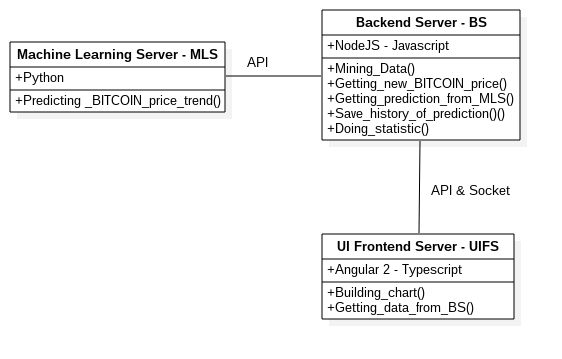
\includegraphics[height=2in, keepaspectratio=true]{system.png}
\caption{Cấu trúc quan hệ và chức năng hệ thống}
\end{figure}
\subsection{Hệ thống máy chủ học máy}
Đây là hệ thống cốt lõi của của sản phẩm, nó đảm nhiệm khối chức năng chính 
liên quan đến các tác vụ học máy, cụ thể, dựa vào các tham số được truyền vào 
để thực hiện quá trình chạy giải thuật dự đoán từ đó đưa ra giá trị nhãn dự 
đoán tương ứng cho bộ tham số đó.\\\\
Hệ thống máy chủ học máy được chia thành hai phần:
\begin{enumerate}
\item Prediction: bao gồm các chức năng đọc mô hình MNN đã xây dựng, chạy mô 
hình với tham số truyền vào và lấy các kết quả đầu ra.Kết quả đầu ra có giá 
trị nhãn $Up-Down$ và xác suất dự đoán.
\item Django: bao gồm các chức năng để trở thành một máy chủ giao tiếp thông 
qua API, các chức năng có thể ví dụ như tiếp nhận các yêu cầu thông qua API, 
phản hồi các yêu cầu dưới dạng các kết quả JSON...
\end{enumerate}
\subsection{ Hệ thống máy chủ backend}
Vì bản thân hệ thống máy chủ học máy không có các khối chức năng liên quan đến 
việc lấy dữ liệu giá BTC cũng như khai phá dữ liệu, nên hệ thống máy chủ backend 
được xây dựng để thực hiện các chức năng này. Đồng thời, máy chủ backend còn là 
cầu nối giữa trải nghiệm người dùng (hệ thống máy chủ UI frontend) và hệ thống 
máy chủ học máy.\\\\
Để thực hiện được công việc trên, hệ thống bao gồm được xây dựng các chức năng:
\begin{enumerate}
\item Cập nhật giá BTC: thông qua các public API được sàn giao dịch Poloniex 
cung cấp, các hàm lấy giá được chạy liên tục để cập nhật giá BTC mới nhất nhằm 
phục vụ cho quá trình dự đoán (trung bình 20 giây).
\item Khai phá dữ liệu: dữ liệu được các hàm cập nhật giá BTC lấy được vẫn 
còn ở dạng thô, chưa qua xử lý. Khai phá dữ liệu là biến đổi các dữ liệu này 
về các bộ tham số có ý nghĩa với Học máy, các giá trị này mới đích thực 
dùng để làm đầu vào dự đoán xu hướng giá trị BTC.
\item Giao tiếp với hệ thống máy chủ học máy: truyền tham số đi và nhận 
kết quả trả về từ hệ thống máy chủ học máy thông qua API.
\item Lưu trữ và thống kê dữ liệu: thực hiện việc lưu trữ dữ liệu, từ đó tạo 
nên một hệ thống các dữ liệu phục vụ cho việc phân tích, thống kê để cung cấp 
cho người dùng đầu cuối. Đó là các thông tin hết sức quý giá phục vụ cho các 
nhà đầu tư.
\item Giao tiếp với hệ thống máy chủ UI frontend: đưa ra những API chức năng 
nhằm phục vụ cho máy chủ UI frontend. Ví dụ như: yêu cầu dữ liệu dự đoán, yêu 
cầu thống kê đúng/sai, yêu cầu dữ liệu giá cho biểu đồ...
\end{enumerate}
\subsection{Hệ thống máy chủ UI frontend}
Hệ thống máy chủ UI frontend là một giao diện người dùng, nó cho phép người 
dùng có thể tiếp cận với các chức năng của toàn bộ hệ thống một cách dễ dàng. 
Hệ thống bao gồm nhiều biểu đồ, cũng như tham số cung cấp các thông tin có ý 
nghĩa đầu tư - dự đoán xu hướng giá trị Bitcoin - đồng thời với đó, là các 
thông tin về độ tin cậy của hệ thống, các thống kê về lịch sử dự đoán...\\\\
Một số hình ảnh về hệ thống thực tế.\\
\begin{figure}[h!]
\centering
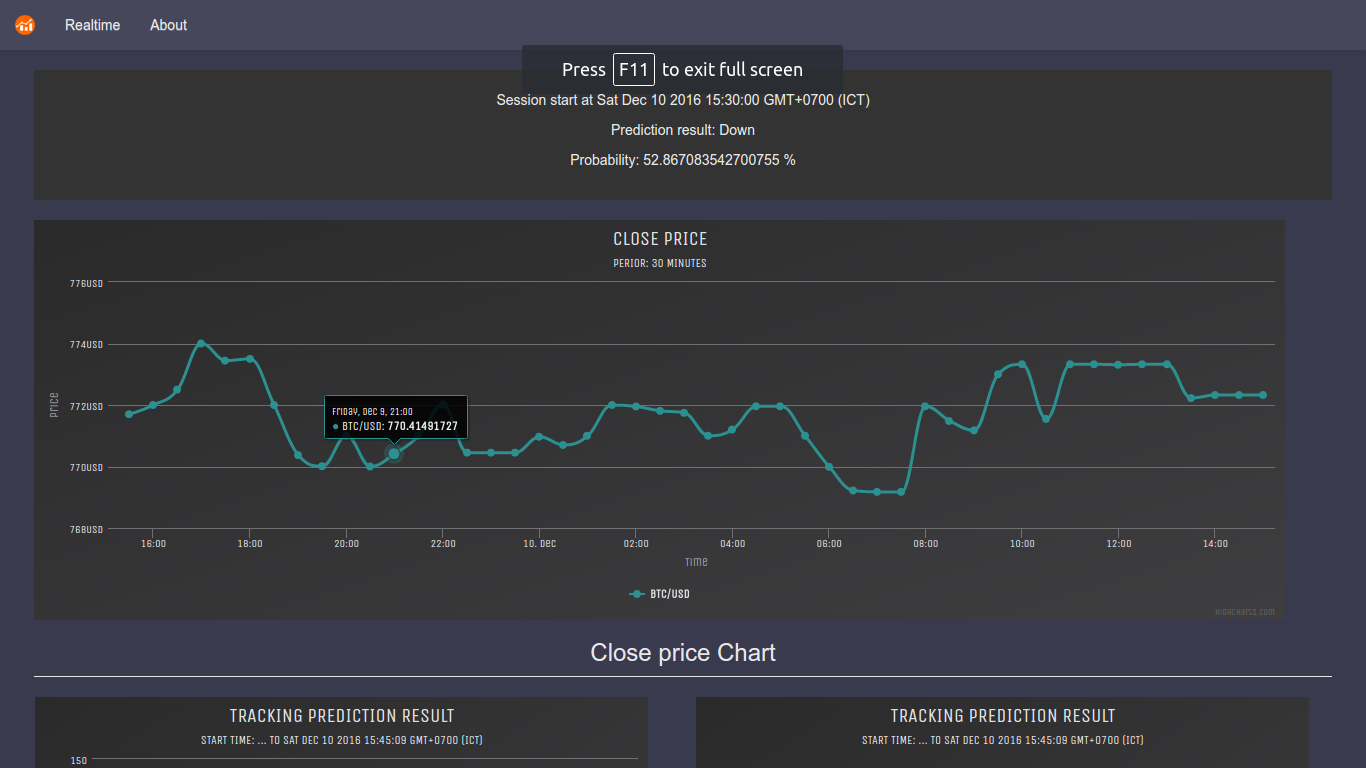
\includegraphics[height=2in, keepaspectratio=true]{2.png}
\caption{Giao diện 2 máy chủ UI frontend}
\end{figure}\\
\begin{figure}[h!]
\centering
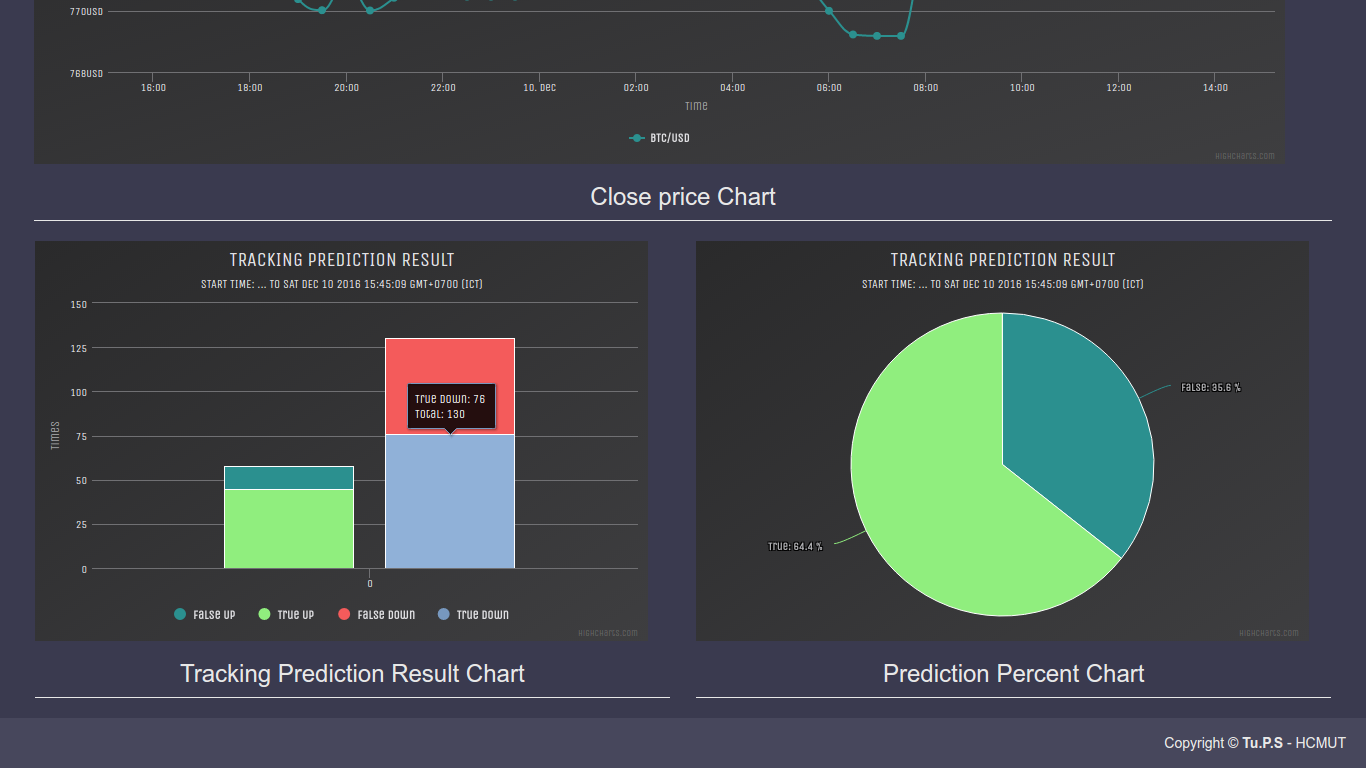
\includegraphics[height=2in, keepaspectratio=true]{3.png}
\caption{Giao diện 3 máy chủ UI frontend}
\end{figure}\\\\